\let\negmedspace\undefined
\let\negthickspace\undefined
\documentclass[journal]{IEEEtran}
\usepackage[a5paper, margin=10mm, onecolumn]{geometry}
%\usepackage{lmodern} % Ensure lmodern is loaded for pdflatex
\usepackage{tfrupee} % Include tfrupee package

\setlength{\headheight}{1cm} % Set the height of the header box
\setlength{\headsep}{0mm}     % Set the distance between the header box and the top of the text

\usepackage{gvv-book}
\usepackage{gvv}
\usepackage{cite}
\usepackage{amsmath,amssymb,amsfonts,amsthm}
\usepackage{algorithmic}
\usepackage{graphicx}
\usepackage{textcomp}
\usepackage{xcolor}
\usepackage{txfonts}
\usepackage{listings}
\usepackage{enumitem}
\usepackage{mathtools}
\usepackage{gensymb}
\usepackage{comment}
\usepackage[breaklinks=true]{hyperref}
\usepackage{tkz-euclide} 
\usepackage{listings}
% \usepackage{gvv}                                        
\def\inputGnumericTable{}                                 
\usepackage[latin1]{inputenc}                                
\usepackage{color}                                            
\usepackage{array}                                            
\usepackage{longtable}                                       
\usepackage{calc}                                             
\usepackage{multirow}                                         
\usepackage{hhline}                                           
\usepackage{ifthen}                                           
\usepackage{lscape}
\begin{document}

\bibliographystyle{IEEEtran}
\vspace{3cm}

\title{NCERT-10.4.3.10}
\author{EE24BTECH11055 - Sai Akhila}
% \maketitle
% \newpage
% \bigskip
{\let\newpage\relax\maketitle}

\renewcommand{\thefigure}{\theenumi}
\renewcommand{\thetable}{\theenumi}
\setlength{\intextsep}{10pt} % Space between text and floats


\numberwithin{equation}{enumi}
\numberwithin{figure}{enumi}
\renewcommand{\thetable}{\theenumi}

% Question
\section*{Question:}
An express train takes $1$ hour less than a passenger train to travel $132$ km between Mysore and Bangalore (without taking into consideration the time they stop at intermediate stations.) If the average speed of the express train is $11$ km/h more than that of the passenger train, find the average speed of the two trains.
%  Solution
\section*{Theoretical Solution:}
Let the speed of the express train be $e$ and the speed of the passenger train be $p$. The time taken by the express train and the passenger train to travel from Mysore to Bangalore would respectively be :\\
\begin{align}
    t_e&=\frac{132}{e}\\
    t_p&=\frac{132}{p}\\
\end{align}
Given that the time taken by express train in 1 hour less,
\begin{align}
    t_p-t_e&=1\\
    \implies \frac{132}{p}-\frac{132}{e}=1
\end{align}
According to the other condition given, 
\begin{align}
    e&=11+p\\
\end{align}
By substituting e in equation $(0.6)$ in equation $(0.5)$, we get:
\begin{align}
    \frac{132}{p}-\frac{132}{11+p}&=1\\
    11\times132&=p^2+11p\\
    p^2+11p-1452&=0\\
    p(p+44)-33(p+44)&=0\\
    (p+44)(p-33)&=0
\end{align}
Hence we get p (the average speed of the passenger train) to be $33$ km/h.\\
The average speed of the express train would be $33+11=44$ km/h
\section*{1. Newton's Method}
Newton's Method is an iterative technique that refines an initial guess \brak{p_0} using the formula:
\begin{align}
    p_{n+1} = p_n - \frac{f\brak{p_n}}{f'\brak{p_n}}.
\end{align}

\subsection*{Advantages}
\begin{itemize}
    \item Quadratic convergence when the initial guess is close to the root.
    \item Requires fewer iterations compared to other methods.
\end{itemize}

\subsection*{Disadvantages}
\begin{itemize}
    \item Requires the computation of the derivative \brak{f'\brak{p}}.
    \item May fail to converge if the initial guess is not close to the root.
    \item Does not guarantee convergence for all functions.
\end{itemize}

\section*{2. Bisection Method}
The Bisection Method is a bracketing method that requires two initial guesses \brak{a} and \brak{b} such that \brak{f\brak{a} \cdot f\brak{b} < 0}. The iterative formula is:
\begin{align}
    p_{n} = \frac{a + b}{2},
\end{align}
where \sbrak{a, b} is updated based on the sign of \brak{f\brak{p_n}}.

\subsection*{Advantages}
\begin{itemize}
    \item Guaranteed convergence if \brak{f\brak{a} \cdot f\brak{b} < 0}.
    \item Simple to implement and does not require the derivative of \brak{f\brak{p}}.
\end{itemize}

\subsection*{Disadvantages}
\begin{itemize}
    \item Convergence is linear, which can be slow compared to Newton's Method.
    \item Requires a bracketing interval \sbrak{a, b} where the root lies.
\end{itemize}

\section*{3. Fixed-Point Iteration}
Fixed-Point Iteration solves equations by rewriting \brak{f\brak{p} = 0} as \brak{p = g\brak{p}} and iterating:
\begin{align}
    p_{n+1} = g\brak{p_n}.
\end{align}

\subsection*{Advantages}
\begin{itemize}
    \item Simple to implement and does not require derivatives.
    \item Useful for equations that can be easily transformed into \brak{p = g\brak{p}}.
\end{itemize}

\subsection*{Disadvantages}
\begin{itemize}
    \item Convergence is not guaranteed unless \brak{|g'\brak{p}| < 1} near the root.
    \item May converge slowly compared to other methods.
\end{itemize}

\section*{ Solving \brak{p^2 + 11p - 1452 = 0}}
The given equation is:
\begin{align}
    p^2 + 11p - 1452 = 0.
\end{align}
We rewrite it as:
\begin{align}
    f\brak{p} = p^2 + 11p - 1452.
\end{align}

\subsection*{Using Newton's Method}
The derivative is:
\begin{align}
    f'\brak{p} = 2p + 11.
\end{align}
The iteration formula becomes:
\begin{align}
    p_{n+1} = p_n - \frac{p_n^2 + 11p_n - 1452}{2p_n + 11}.
\end{align}

\subsection*{Using Bisection Method}
Choose \sbrak{a, b} = \sbrak{30, 40}, since \brak{f\brak{30} < 0} and \brak{f\brak{40} > 0}. The iterative formula is:
\begin{align}
    p_{n} = \frac{a + b}{2}.
\end{align}
Update \brak{a} or \brak{b} based on the sign of \brak{f\brak{p_n}}.

\subsection*{Using Fixed-Point Iteration}
Rewrite the equation as:
\begin{align}
    p = g\brak{p} = \sqrt{1452 - 11p}.
\end{align}
The iteration formula is:
\begin{align}
    p_{n+1} = \sqrt{1452 - 11p_n}.
\end{align}
Convergence depends on the initial guess and the condition \brak{|g'\brak{p}| < 1}.

\section*{5. Ideal Method for \brak{p^2 + 11p - 1452 = 0}}
Given the nature of the equation:
\begin{itemize}
    \item Newton's Method is ideal if a good initial guess is available, as it converges rapidly.
    \item Bisection Method is robust and guarantees convergence but is slower.
    \item Fixed-Point Iteration is less reliable and may require careful transformation to ensure convergence.
\end{itemize}
Newton's Method is recommended for this problem due to its efficiency.

\section{Using Newton's method along with bisection method for improved efficiency}
Now, we solve the quadratic equation
\begin{align}
p^2 + 11p - 1452 &= 0
\end{align}
using a combination of Newton's method and the bisection method. While Newton's method is efficient and converges rapidly when close to the root, it can fail if the initial guess is far from the root or if the derivative is zero. The bisection method is slower but more robust, ensuring convergence as long as the function changes sign over an interval. By combining both methods, we achieve the robustness of the bisection method and the speed of Newton's method.


\subsection{Combining the Methods}
To combine these methods, we proceed as follows:
\begin{enumerate}
    \item Use the bisection method to narrow the initial interval where the root is likely to be located.
    \item Once the interval is sufficiently small, apply Newton's method to converge more rapidly to the root.
    \item If Newton's method diverges or does not converge, fall back to the bisection method to refine the root estimate.
\end{enumerate}

This strategy ensures that the method remains robust and guarantees convergence, while taking advantage of the faster convergence rate of Newton's method.

\subsection{Results}
We applied the combined method to the quadratic equation \( p^2 + 11p - 1452 = 0 \) with an initial interval \([-50, 33]\). The method successfully converged to the root, demonstrating the effectiveness of combining the robustness of the bisection method with the fast convergence of Newton's method.


\section{Solving using eigen values:}
Alternatively, we can solve the question by using the eigen values of the companion matrix.\\
For a polynomial equation of form $x^n+c_{n-1}x^{n-1}+\dots+c_2x^2+c_1x+c_0 = 0$ the companion matrix is of the form:
\begin{align}
	\myvec{
		0 & 0 & \cdots & 0 & -c_0\\
		1 & 0 & \cdots & 0 & -c_1\\
		0 & 1 & \cdots & 0 & -c_2\\
		\vdots & \vdots & \ddots & \vdots & \vdots\\
		0 & 0 & \cdots & 1 & -c_{n-1}\\
	}
\end{align}
The eigen values of this matrix are the roots of the polynomial equation. For this question,
\begin{align}
	n &= 2\\
	c_0 &= -1452\\
	c_1 &= 11\\
	C &= \myvec{0 & 1452 \\ 1 & -11}
\end{align}
The QR algorithm is an iterative method used to find the eigenvalues of a square matrix. It is based on decomposing a matrix into its QR decomposition (where Q is an orthogonal matrix and R is an upper triangular matrix), and then iteratively improving the approximation of the eigenvalues.
\subsection{The Gram-Schmidt orthogonalization}
Consider a matrix A. It can be represented as 
\begin{center}
    $A=\left[\vec{a_1} \vec{a_2}....\vec{a_3}\right]$
\end{center}
$\tilde{q}_1 = \vec{a_1}$, $\vec{q_1}=\frac{\tilde{q}_1}{\|\tilde{q}_1\|}$\\
$\tilde{q}_2 = \vec{a}_2 - (a_2^T\vec{q_1})\vec{q_1}$\\
$\vec{q_2}=\frac{\tilde{q}_2}{\|\tilde{q}_2\|}$\\
\textbf{Generalising the algorithm:}\\
Intialise $\tilde{q}_1=\vec{a_1}$, $\vec{q_1}=\frac{\tilde{q_1}}{\|\tilde{q_1}\|}$\\
for r=2 to k:\\
\begin{center}
$\tilde{q_r} = \vec{a_r} - $\(\sum_{i=1}^{r-1} (a_r^Tq_i)q_i\)\\
$\vec{q_r}=\frac{\tilde{q}_r}{\|\tilde{q}_r\|}$
\end{center}
Hance, we can write any matrix A as: 
\begin{center}
A = QR\\

\end{center}
where Q is the orthogonal matrix that consists of orthogonal basis of A, and image space of A = image space of Q.
R is an upper triangular matrix, whose diagonal entries are the norms of the respective column vectors and the upper diagonal entries are dots products of the corresponding vectors with the orthogonal vectors in Q (in the indices less than the corresponding index).
\subsection{Hessenburg reduction:}
To reduce a matrix A to Hessenberg form, the Householder transformations are commonly used. The process works by successively applying orthogonal transformations to eliminate the elements below the first sub-diagonal.\\
Householder transformations are used to create zeros below the diagonal and the first subdiagonal of the matrix. The goal is to zero out the entries $A_{i,j}$ for $i>j+1.$\\
The Householder transformation is a reflection operation that transforms the given matrix by applying orthogonal matrices to it. A Householder matrix H is constructed as:
\begin{center}
  $H=I-2\frac{\vec{v}\vec{v}^T}{\vec{v}^T\vec{v}}$
\end{center}

where $\vec{v}$ is a vector that reflects the given column vector $\vec{x}$ (the portion of the matrix you want to zero out) to align with a scalar multiple of a unit vector. This is done repeatedly for each column, creating the Hessenberg form.\\
Repeat for all columns.\\
After applying the transformations, the result will be an upper Hessenberg matrix where all elements below the first sub-diagonal are zero.\\


\subsection{Iterating the QR decomposition:}
\begin{enumerate}
    \item Perform QR decomposition $A_k=Q_kR_k$
    \item Compute the next matrix $A_k+1=R_kQ_k$
    \item Repeat the process until $A_k$ converges to a nearly upper triangular matrix 
    \item The diagonal entries of the converged matrix are the eigenvalues of A.
\end{enumerate}
\section{Time Complexity:}
The time complexity of the QR algorithm primarily depends on two factors:
\begin{enumerate}
    \item The number of iterations required for convergence
    \item The computational cost of each iteration
\end{enumerate}
The total time complexity of the QR algorithm is the product of the cost of one QR decomposition and the number of iterations:
\begin{enumerate}
    \item \textbf{Per iteration}: QR decomposition costs O($n^3$)(using Gram-Schmidt algorithm)
    \item \textbf{Number of iterations}: The algorithm typically converges in O(n) iterations.
\end{enumerate}
Thus, the overall time complexity of the QR algorithm is:
\begin{center}
    $O(n^3)\times O(n)=O(n^4)$
\end{center}
For optimized version\textbf{(Hessenburg reduction)}:
The matrix is often reduced to Hessenberg form (H) using a pre-processing step that costs O($n^3$).\\This reduces the cost of the QR decomposition to O($n^2$) for Hessenberg matrices.\\
Time complexity with Hessenberg reduction: O($n^3$) for reduction + O($n^2$) per iteration $\implies$ Overall complexity: O($n^3$)

\begin{figure}[h!]
    \centering
    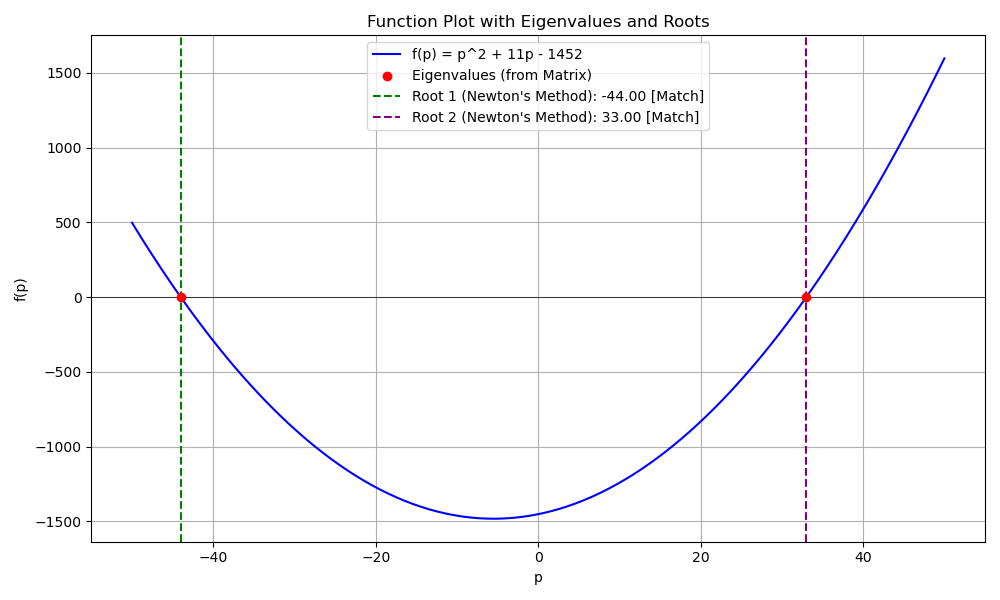
\includegraphics[width=\columnwidth]{figs/e.png} % Replace with your image filename
    \caption{Eigenvalues and Roots Highlighted}
    \label{fig:eigenvalues_roots}
\end{figure}

\end{document}





